\chapter{Dataset}\label{chapter:Dataset}
%TODO: ++ Add visualisations of samples I guess
%TODO: add overview for patch options from presentation in drive!
\section{Training Dataset}

The dataset we used for training is a synthetic dataset created with Blenderproc \cite{denninger2019blenderproc}. It consists of scenes of 10 subsequent frames from different vantage points. In total we have 900 sequences we used for training and 89 for during training validation. During the dataset generation, different camera movements were simulated, resulting in object occlusions. As a result, the classes encountered in one sequence may not be present in each individual frame of the sequence. \par
% maybe add more details on camera movement and dataset creation if asked
% how many data and how organised?

During training, we'd like to have the option to load a sequence of neighboring frames and their annotations with every call of the \_\_get\_item() method in the dataloader. Our dataset consists of sequences of 10 frames, but in practice we'd like to have the option to load shorter sequences sampled from the 10 frame sequences. \par 

Another important aspect for dataloading is the patch generation within a sequence. In practice, we examined two options for patch generation:
\begin{itemize}
    \item Case 1: The first patch in the sequence is generated from the corresponding ground truth masks and the next from the predictions. The dataloader only needs to return the patches for t=0 in the sequence, the next patches are generated during training in the forward() method of our model. Typical sequence length in that case is T=3.
    \item Case 2: The first and potentially any other patches depending on the sequence length are generated from neighboring frames. Typical sequence length in that case is T=1. 
\end{itemize}

Depending on the patch generation approach and the sequence length, the \_\_get\_item() method returns a batched sequence of images and their respective ground truth masks as well as one (case 1) or multiple (as many as the input image sequence length) patches generated in the way explained above.

\begin{table}[htpb]
  \caption[Dataloading explained]{Possible frame sequences in the dataloading process}\label{tab:dataloading}
  \centering
  \begin{tabular}{ |p{0.6cm}|p{0.2cm}|p{0.2cm}|p{0.2cm}|p{0.2cm}|p{0.2cm}|p{0.2cm}|p{0.2cm}|p{0.2cm}|p{0.2cm}|p{0.2cm}|p{0.2cm}|p{0.2cm}|p{0.2cm}|p{0.2cm}|p{0.2cm}|p{0.2cm}|p{0.2cm}|p{0.2cm}|p{0.2cm}|p{0.2cm}| }
 \hline
 \multicolumn{11}{|c|}{frame id} \\
 \hline
% \multirow{5}{}{}
   t=0 & 0 & 1 & 2 & 3 & 4 & 5 & 6 & 7 & 8 & 9\\
 \hline
  t=1 & 1 & 2 & 3 & 4 & 5 & 6 & 7 & 8 & 9 & 0\\
  \hline
  t=2 & 2 & 3 & 4 & 5 & 6 & 7 & 8 & 9 & 0 & 1\\
 \hline

\end{tabular}
\end{table}


The input images are not augmented, because adding random noise or flipping them increases the differences between neighboring frames to a level that doesn't help the model recognise the same object in different sequences. In general, we'd like to keep the difference betweeen frames minimal for training, simulating small and rather smooth movements of the camera. The only processing taking place with regard to the input images is a normalisation.\par
Though the images are not augmented, there's an option to augment the tracks by sampling neighboring frames more freely in the sequence. In practice, we use this track augmentation in the second case of patch generation. \par


\begin{figure}
\caption{Dataset sequence with smooth movement without occlusions}
\centering
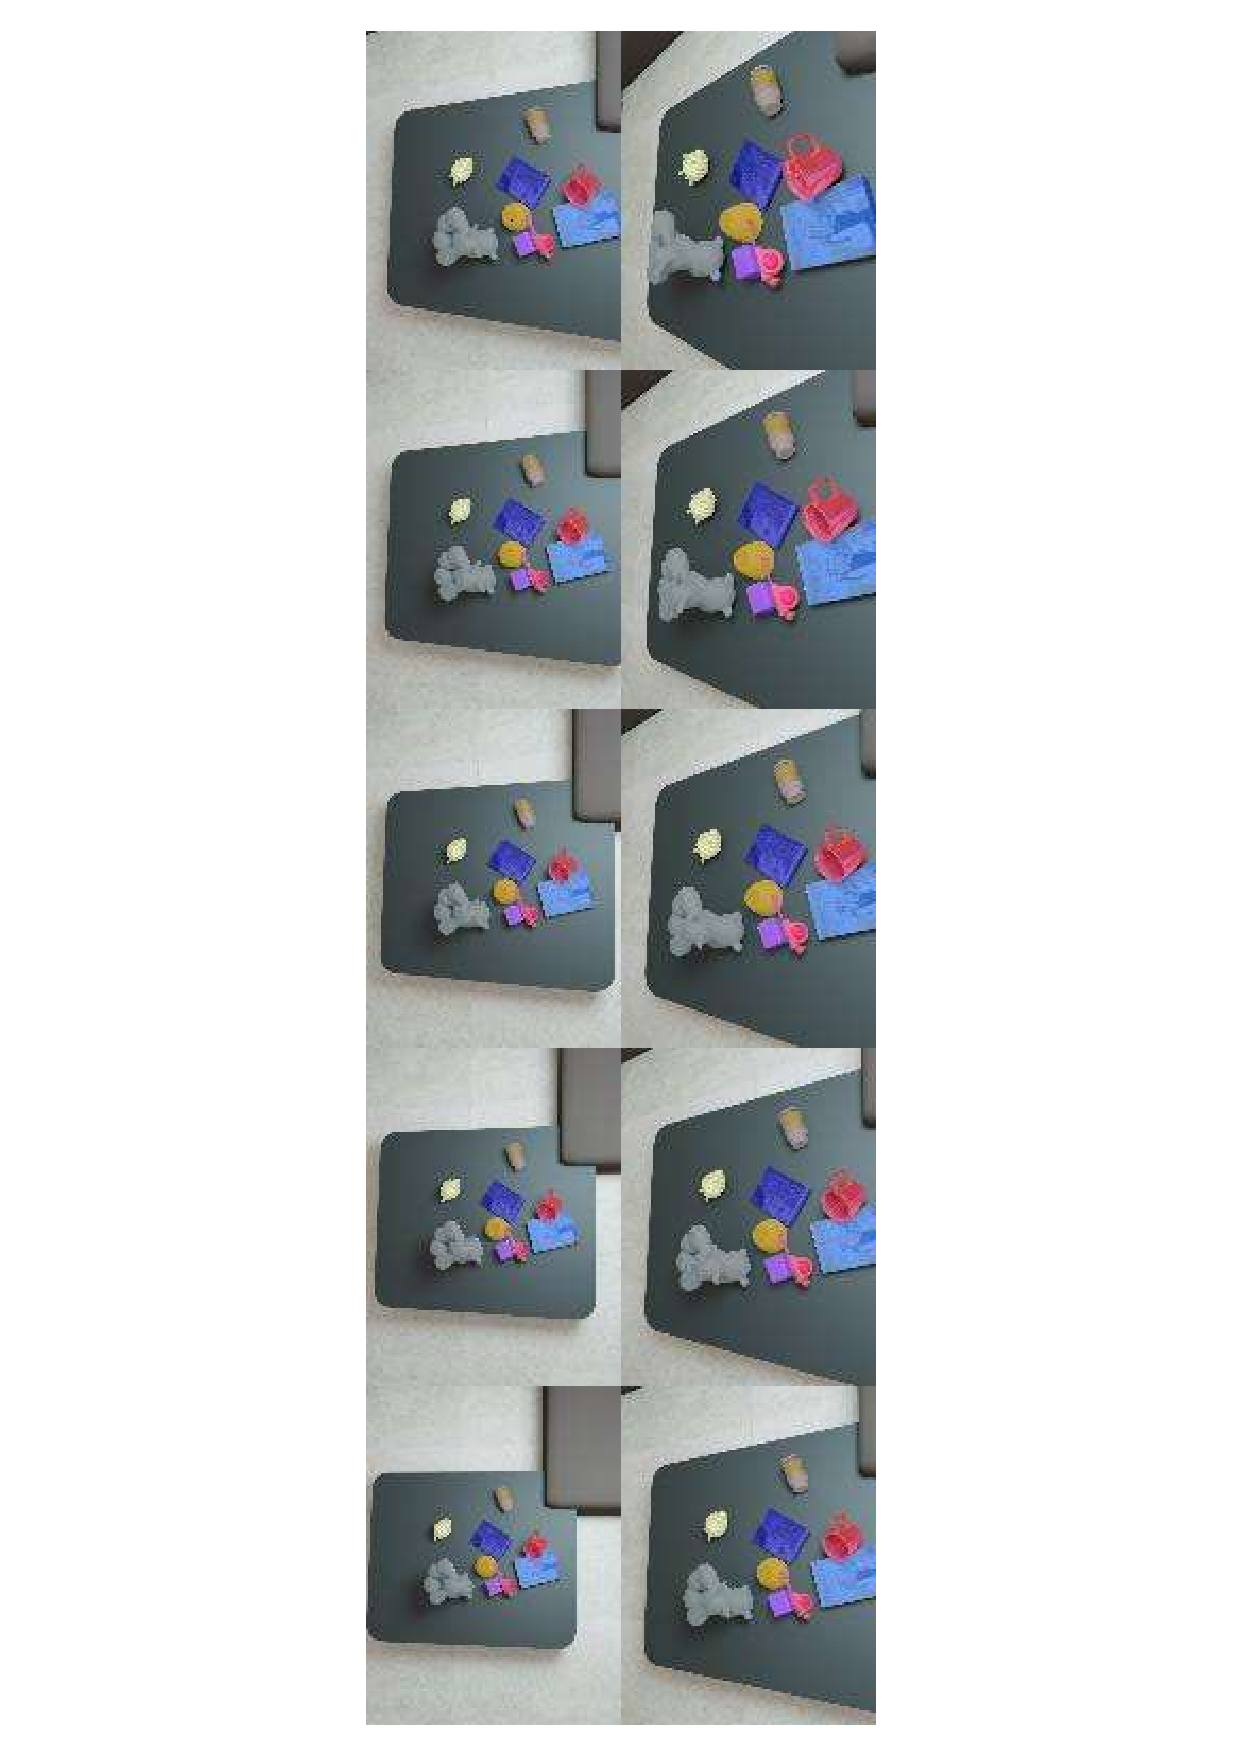
\includegraphics[width=0.9\textwidth]{figures/dataset.jpg}
\end{figure}

\begin{figure}
\caption{Dataset sequence with more abrupt movement that results in occlusions}
\centering
\includegraphics[width=0.9\textwidth]{figures/dataset_occlusions.jpg}
\end{figure}

\section{Two approaches in patch generation}
%This could also be moved in the dataset
\textbf{Approach A: use preds to generate patches}\\
* gt\_t0 -> patches\_t0
* pred\_t0 -> patches\_t1
* pred\_t1 -> patches\_t2
\textbf{Approach B: only use ground truths to generate patches}\\
* gt\_t3 -> patches\_t0
* gt\_t4 -> patches\_t1
* gt\_t5 -> patches\_t2

gt\_t3-5 are sampled from within the same sequence (not necessarily frame 3 in sequence, just using the different indices to emphasize that they are different than the gts 0,1,2 with the annotations for input ims 0,1,2. So always using different neighboring gts to generate the patches. Their total number is related to the sequence length we are training on. For T=1 gt1-> patches0 for im0 with gt0!
